\chapter{European Spallation Source and beam diagnostic devices}
\chaptermark{European Spallation Source and beam diagnostic devices}
\cleardoublepage

\minitoc
\section{Introduction}
\begin{refsection}
  \label{ch2:Introduction}
  This thesis deals about the design of non-invasive ionization profilers for the ESS proton beam. To produce neutrons, the European Spallation Source (ESS) will be based on one of the most powerful linear proton accelerators ever built. Therefore, the beam diagnostic is an important part of the project to insure the safety of the machine during the commissioning and the operation.

  This chapter gives an overall vision of the ESS project. The different elements of the accelerator will be briefly detailed from the source to the target. In addition, some neutron instruments foreseen at ESS and their applications will be illustrated.

  The second part of the chapter focuses on beam diagnostic devices and their diversity. An exhaustive list of beam diagnostics is not possible and so only few of them are presented here. The chapter concludes with the state of the art of non-invasive profilers based on the ionization of residual gas.

  \section{Beam dynamic}
  \section{European Spallation Source}
  \begin{figure}[!ht]
  \begin{center}
    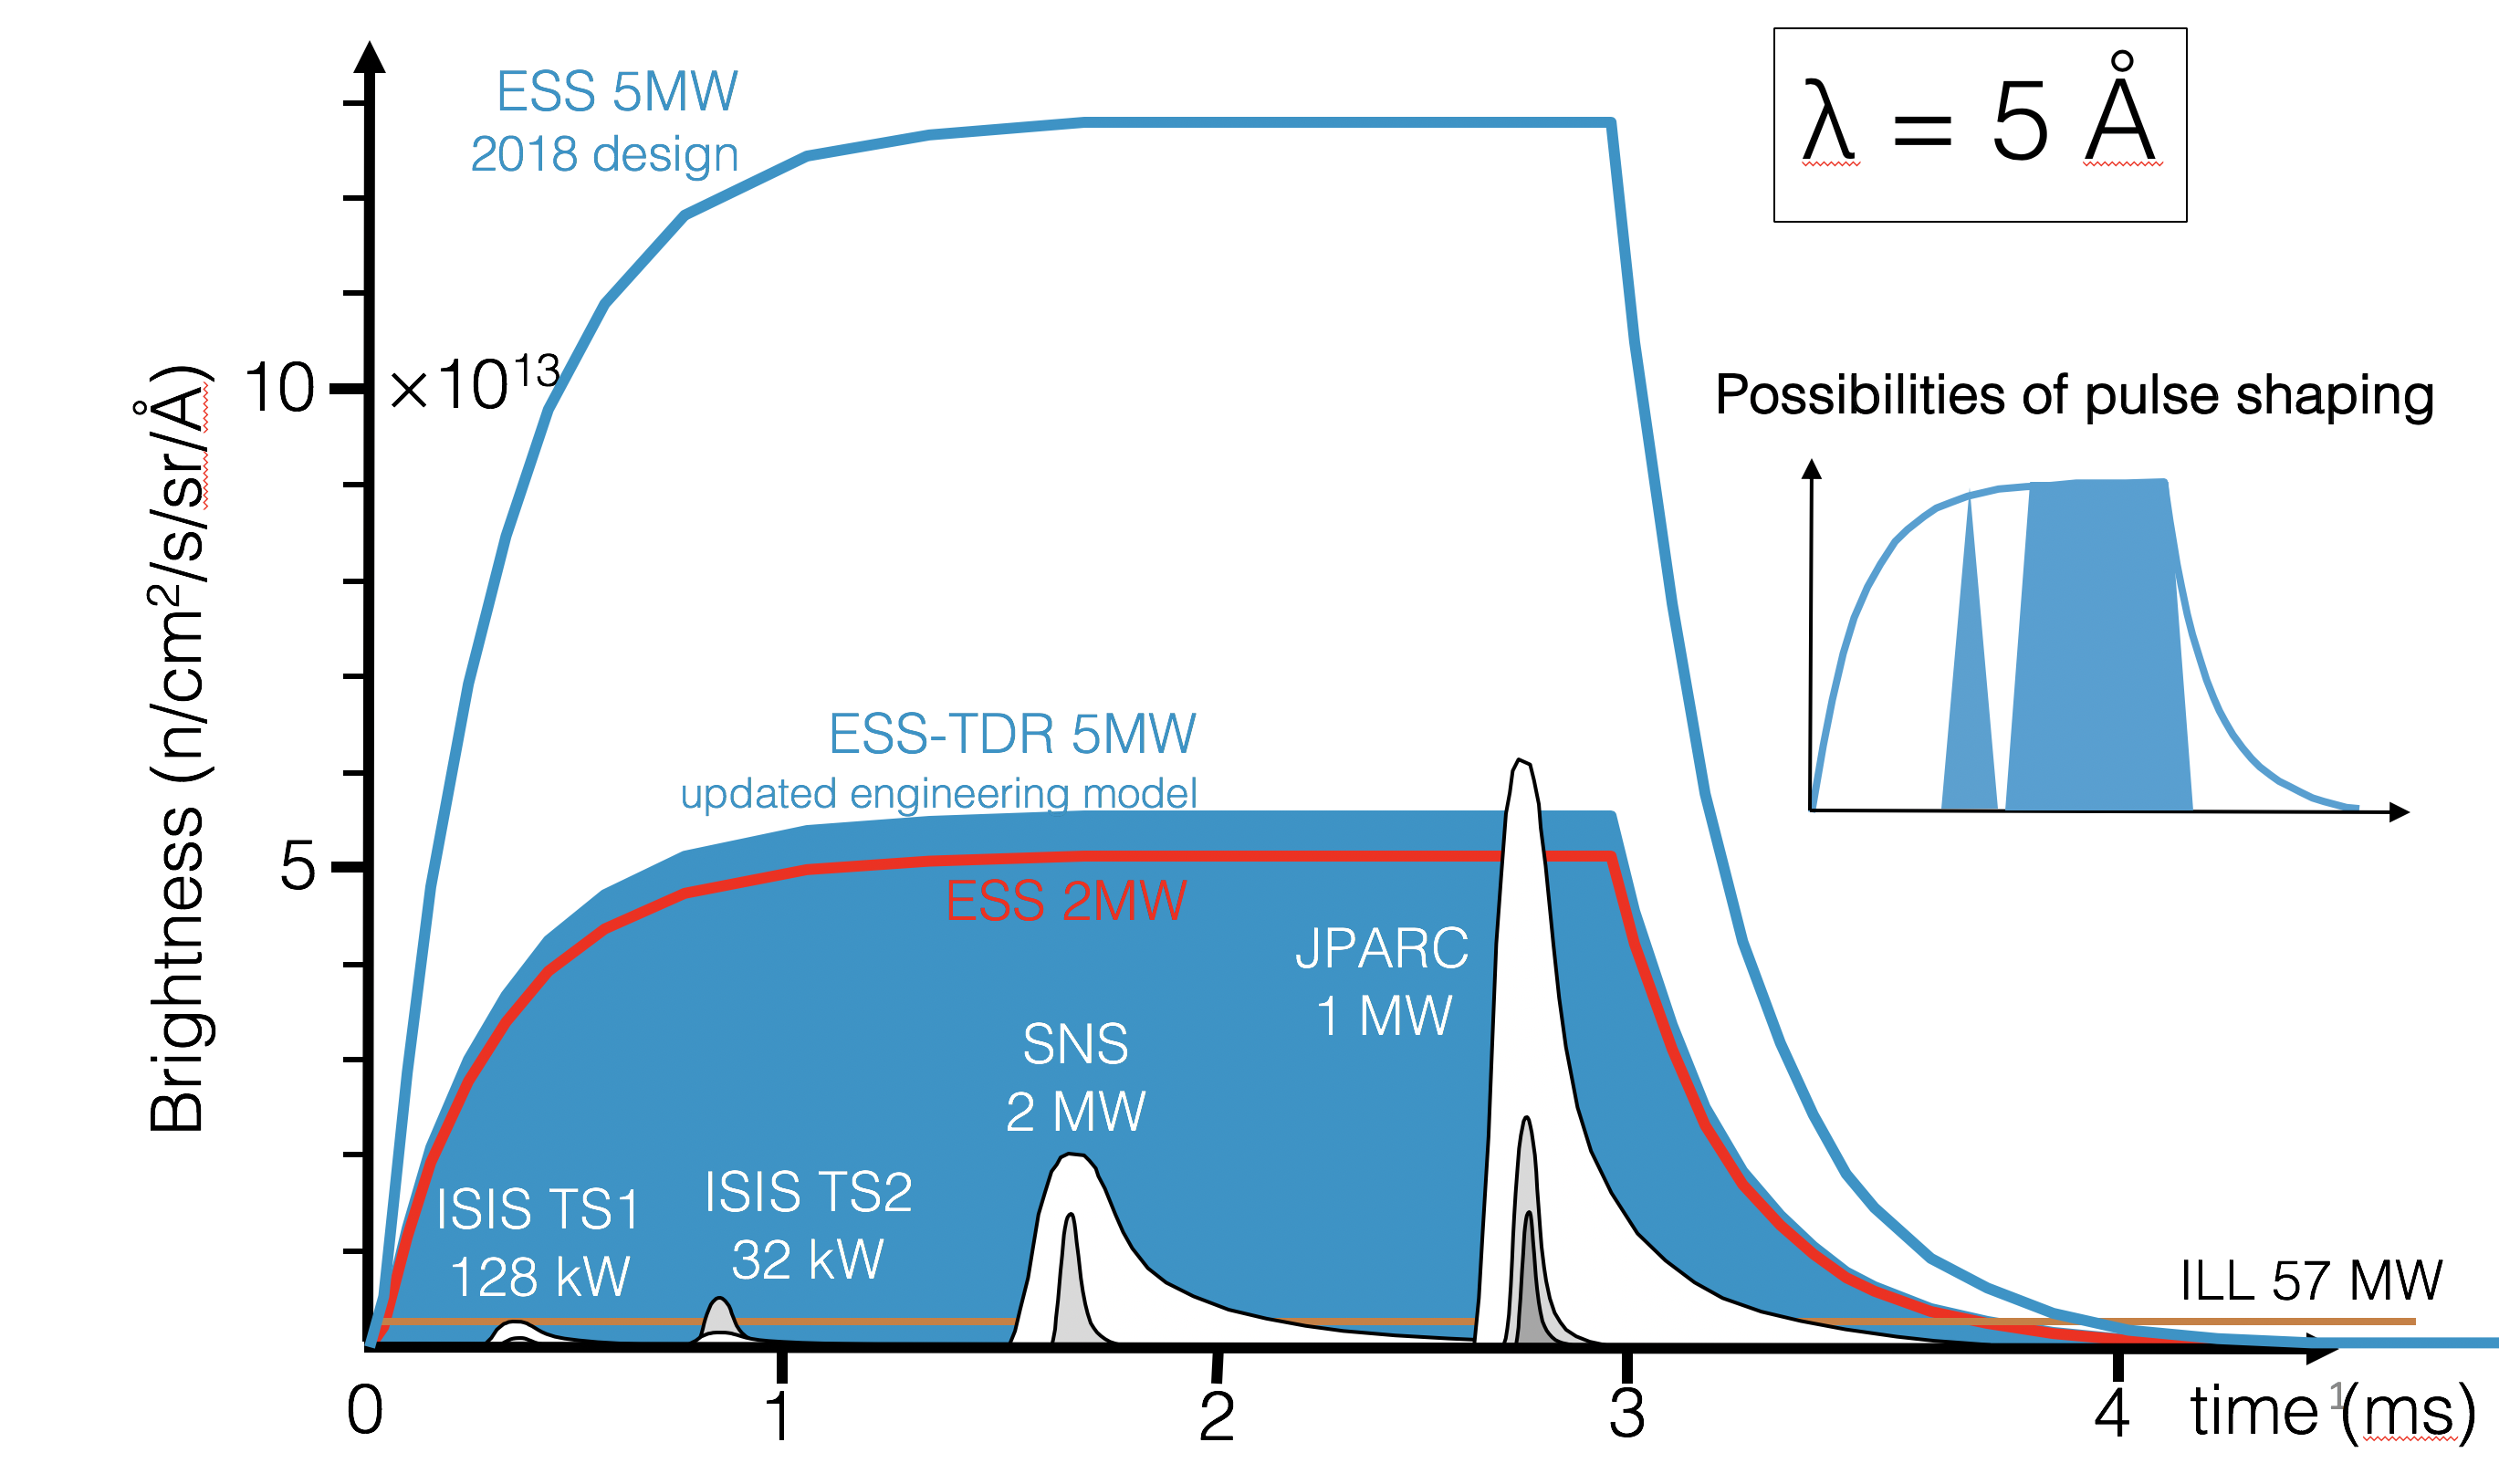
\includegraphics[width=\textwidth]{02_BeamDiag/figures/fig000_ESS_pulse}

  \end{center}
  \caption[ESS neutron source brightness compared to others existing neutron sources]{ESS neutron source brightness compared to others existing neutron sources.}
  \label{chap3:fig:ESS_pulse}
\end{figure}


  \section{ESS collaboration and ESS activities at CEA/IRFU}



  \section{ESS accelerator}
  The proton linear accelerator (LINAC or linac) of ESS is represented synthetically in Fig. \ref{chap2:fig:ESS_acc}.
  The total length from source to target is about $600\,\mathrm{m}$ and $356\,\mathrm{m}$ are dedicated to the acceleration. The first part accelerates the beam up to $90\,\mathrm{MeV}$ by mean of conventional room temperature RF cavities. Then a cold part using superconducting cavities cooled with liquid helium is used to reach the highest energies.

  \begin{figure}[!ht]
	\begin{center}
		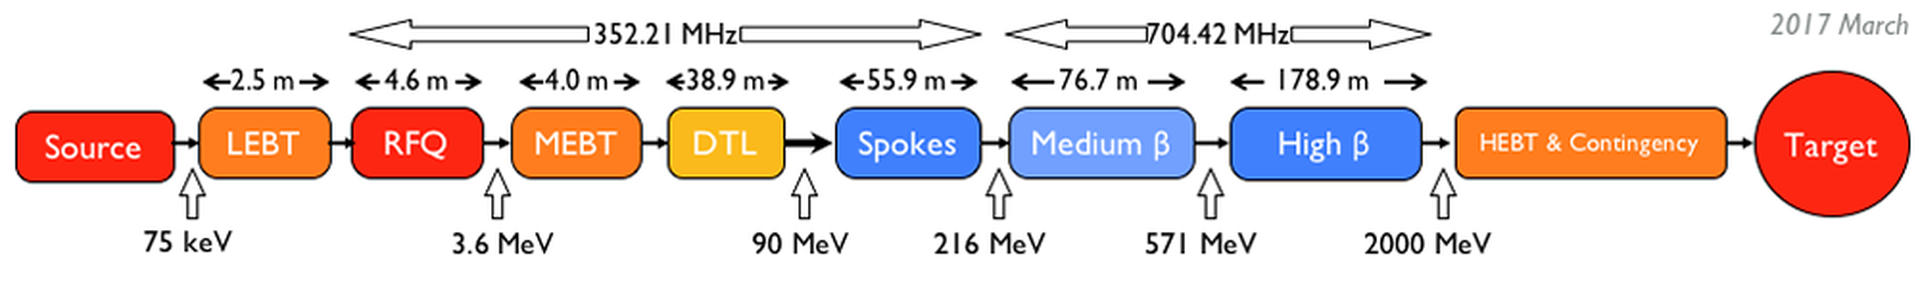
\includegraphics[width=\textwidth]{02_BeamDiag/figures/fig000_ESS_acc}
	\end{center}
	\caption[A simplified representation of the ESS linac]{A simplified representation of the ESS linac. Blue blocks represent superconducting cavities where IPMs will be installed.}
	\label{chap:}
\end{figure}


  Table \ref{chap2:tab:ess_charac} summarizes the most important characteristics of the ESS linac. The particularities of ESS compared to other sources of spallation are its very long pulse and its high current. The average beam power is 5 MW and th peak power is 125 MW, making ESS one of the most powerful proton accelerators in the world.

  \begin{table}[ht]
  \centering
  \caption[ESS nominal conditions]
  {ESS nominal conditions.}
  \label{chap2:ess_charac}
  \begin{tabular}{ll}
    \toprule
    Characteristic    & Value                  \\
    \midrule
    Energy            & $2\,\mathrm{GeV}$      \\
    Current           & $62.5\,\mathrm{mA}$    \\
    Pulse duration    & $2.86\,\mathrm{ms}$    \\
    Power             & $5\,\mathrm{MW}$       \\
    Repetition rate   & $14\,\mathrm{Hz}$      \\
    Duty cycle        & $4\,\mathrm{\%}$       \\
    Radio Frequencies & $352.21\,\mathrm{MHz}$ \\
                      & $704.42\,\mathrm{MHz}$ \\
    \bottomrule
  \end{tabular}
\end{table}

  In the following sections the role of each of the accelerator blocks is described.

  \subsection{Ion source and Low Energy Beam Transport}

  \subsection{Radio Frequency Quadrupole}
  The principle of the Radio Frequency Quadrupole (RFQ) was imagined in the 1970s in Russia by Kapchinskiy and Tepliakov. The method has quickly become popular and indispensable in very intense accelerators since it still the most efficient method of acceleration at low energies.

  At these energies, the space charge is so high that the beam divergence is enormous and must be compensated. An RFQ behaves as a sequence of focusing and defocusing elements that can contain the space charge. RF waves are propagated on four poles (usually vanes or rods) with opposite amplitude between each pole. The RF variation allows to successively focus in one direction (and defocus in the other direction). A mechanical modulation of the vanes introduces a longitudinal electric field that will accelerate the particles. In concrete terms, an RFQ:
  \begin{itemize}
    \item contains and focuses the beam.
    \item accelerates the particles
    \item structures the beam into small bunches
  \end{itemize}

  Simulations of such device are complicated required specific codes to compute the propagation of the RF waves and the transport of particles inside the RFQ \cite{Duperrier2000}. As well, the conception of this type of cavities is extremely technical, for instance the tolerance on the mechanical structures of the vanes is in the order of micrometers whereas the whole RFQ structure often exceeds meters.

  The CEA/IRFU is in charge of the construction of the ESS RFQ \cite{ChirpazIPAC2016} which accelerates the proton at the source output to $3.6\,\mathrm{MeV}$ and bunches them with a $352.21\,\mathrm{MHz}$ frequency.

  \subsection{Medium Energy Beam Transport}

  \subsection{Drift Tube Linac}

  \subsection{Superconducting cavities}
  \begin{figure}[!ht]
	\begin{center}
		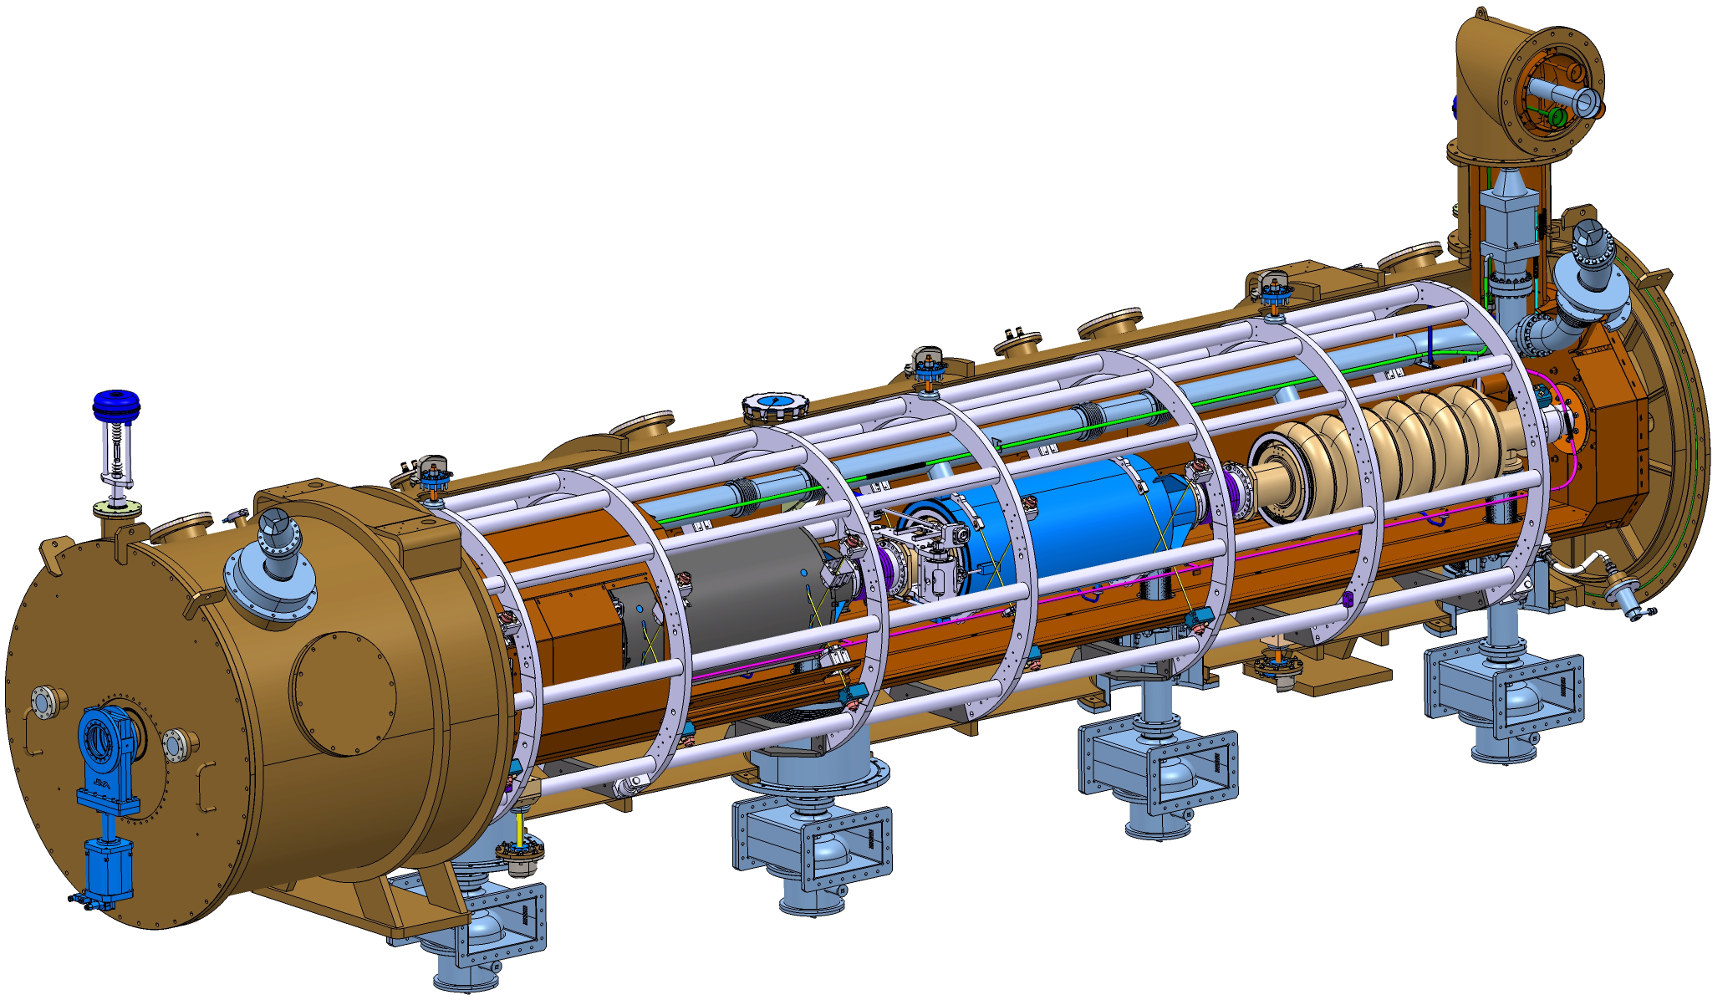
\includegraphics[width=\textwidth]{02_BeamDiag/figures/fig000_cryo_a2}
	\end{center}
	\caption[ESS medium beta elliptical cavities cryomodule]{ESS medium beta elliptical cavities cryomodule.}
	\label{chap2:fig:ESS_cryo}
\end{figure}


  \subsection{Transport lines}
  \section{Target}
  \section{Instruments}

  \section{Beam diagnostic overview}
  \subsection{Beam position monitor}
  \subsection{Beam current monitor}
  \subsection{Beam loss monitor}
  \subsection{Beam emittance measurements}
  \section{Invasive beam profile measurements}
  \subsection{Interceptive screen}
  \subsection{Grid profiler}
  \subsection{Wire scanner}
  \section{Non-invasive beam profile measurements}
  \subsection{Laser wire profiler}
  \subsection{Beam induced fluorescence profiler}
  \section{Ionization Profile Monitor and summary}
  \label{ch2:Summary}

  \cleardoublepage
  \section*{Bibliography}
  \addcontentsline{toc}{section}{Bibliography}
  \label{ch2:bib}
  \printbibliography[heading=subbibliography]

\end{refsection}